\documentclass{article} 
\usepackage{amssymb, amsfonts, amsmath, amsthm}
\usepackage{epsfig,lpic,wrapfig}
\usepackage{fontawesome}
\usepackage[T2A,T1]{fontenc}
\usepackage[utf8]{inputenc}
\usepackage[english,russian]{babel}
\usepackage{graphicx}
\usepackage{url}
%\usepackage[top=0.9in, bottom=0.9in,left=0.9in, right=0.9in, paperwidth=6in, paperheight=9in]{geometry}
\usepackage[colorlinks=true,
citecolor=black,
linkcolor=black,
anchorcolor=black,
filecolor=black,
menucolor=black,
urlcolor=black%
]{hyperref}
\hypersetup{pdftitle={Блуждания с Марковым},
pdfauthor={Александр Гиль и Антон Петрунин}}



\begin{document}
\title{Блуждания с Марковым}
\author{А. Гиль и А. Петрунин}
\date{}
\maketitle
\begin{abstract}
Заметка основана на лекции прочитанной первым автором в школьном 
математическом кружке Northwest Academy of Science.
\end{abstract}

\section{Вероятность и математические ожидание}

Подкидывая кубик,
с равными шансами мы можем получить 1, 2, 3, 4, 5 или 6 очков.
Результат такого \emph{испытания} --- число очков, выпавшее на 
верхней грани кубика является простым примером \emph{случайной величины}.
Естественно предположить, что результат одного испытания (подкидывания кубика)
не зависит от других таких же испытаний.


Давайте записывать значения нашей случайной величины, много раз подкидывая кубик,
и вычислять долю испытаний, давших конкретный результат (например, 5 очков) среди всех наших испытаний.
При увеличении числа испытаний до бесконечности эта доля стремится к пределу, 
который называется \emph{вероятностью} этого исхода.
Поскольку шансы любого из шести исходов равны, вероятность каждого исхода равна $\tfrac16$.

Давайте теперь не только записывать результат каждого испытания, но и считать среднее
арифметическое всех записанных на данный момент результатов. Если эта последовательность стремится к
определённому числу, то такое число называется \emph{математическим ожиданием} или \emph{средним значением}
случайной величины.

В нашем примере искомое среднее значение 
числа очков можно посчитать по формуле
\[\tfrac16\cdot1+\tfrac16\cdot2+\tfrac16\cdot3+\tfrac16\cdot4+\tfrac16\cdot5+\tfrac16\cdot6=3\tfrac12.\]
Действительно, в пределе на долю каждого исхода 1, 2, 3, 4, 5 и 6
приходится $\tfrac16$ числа всех исходов, и, значит, их среднее арифметическое должно 
стремиться к левой стороне равенства.

Иначе говоря, для вычисления среднего значения мы должны вычислить \emph{взвешенную сумму} значений нашей величины
для каждого исхода (1, 2, 3, 4, 5 и 6), взяв вероятность каждого исхода ($\tfrac16$) в качестве веса.

\medskip

Несмотря на очевидность высказанных выше утверждений,
чтобы придать им точный математический смысл,
требуется развить неболшую теорию, которую остаётся за рамками нашей заметки.
Мы обсудим только способы нахождения вероятностей и средних значений в чуть более сложных ситуациях.

Вообще говоря, может оказаться, что среднее значение (математическое ожидание), вычисляемое как предел для продлеваемой бесконечно серии испытаний, не существует для данной схемы испытаний. 
Такое может случится,
поскольку у бесконечной последовательности чисел предельного значения может не существовать.

Популярным примером ситуации без предельного значения является так называемый «Санкт-Петербуржский парадокс». 
В наших задачах такого происходить не будет,
но мы не будем это строго доказывать.

\section{Робот Чебуратор на коротком столе} 

Электромеханическая игрушка «Робот Чебуратор», 
будучи включенной, через равные интервалы времени делает шаги одинаковой длины налево или направо,
выбирая между этими двумя направлениями с одинаковой вероятностью $\tfrac12$.

{

\begin{wrapfigure}{r}{17 mm}
\begin{lpic}[t(10 mm),b(0 mm),r(0 mm),l(2 mm)]{pics/stol(.35)}
\lbl[b]{15,11;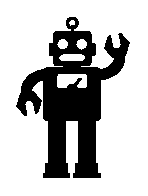
\includegraphics[scale=.7]{pics/robot}}
\end{lpic}
\end{wrapfigure}

Предположим, Чебуратор стоит на левом краю короткого стола: шагая влево, он чебурахнется со стола.
Однако, он может шагнуть вправо и остаться на столе (на правом краю) --- но он чебурахнется после второго
шага направо. 
Нас интересуют следующие две задачи.

}
\begin{itemize}
\item Какова вероятность того, что робот чебурахнется с левого края стола, и какова --- что с правого?
\item Чему равно среднее значение числа шагов которые, сделает робот, чтобы чебурахнуться?
\end{itemize}
При этом мы полагаем, что существование требуемых чисел в обоих вопросах обосновано
(это действительно верно, хотя требует доказательства); нам остаётся лишь найти их численные значения.

\medskip
\noindent\textit{Решение первой задачи.}
Пусть $p_1$ и $p_2$ обозначают вероятность чебураханья из первого (левого) и второго (правого) положения.
Заметим, что
\[p_1=\tfrac12\cdot0+\tfrac12\cdot p_2.\]
Действительно, после первого шага с вероятностью $\tfrac12$ робот чебурахнется налево,
и, значит, шансов чебурахнуться направо у него уже не будет, 
отсюда слагаемое $0=\tfrac12\cdot0$. С той же вероятностью он перейдёт на второе место,
откуда у него будет вероятность $p_2$ чебурахнутся вправо, отсюда слагаемое $\tfrac12\cdot p_2$.

Аналогично получаем уравнение 
\[p_2=\tfrac12\cdot p_1+\tfrac12\cdot 1.\]
Эти два уравнения говорят, что в последовательности из четырёх чисел
\[0,\  p_1,\  p_2,\ 1\]
каждое является средним арифметическим своих соседей.
Иначе говоря, эта последовательность является арифметической, 
и, значит, $p_1=\tfrac13$ и $p_2=\tfrac23$.

Заметим, что если $q_1$ и $q_2$ вероятности чебураханья налево, 
то, повторив те же вычисления, получаем $q_1=\tfrac23$ и $q_2=\tfrac13$.
Этот же результат можно получить, посмотрев на задачу через зеркало, меняющее местами право и лево.

В частности, из положения 1, робот чебурахается направо и налево с вероятностями $\tfrac13$ и $\tfrac23$.
Заметим, что 
\[p_1+q_1=p_2+q_2=1,\]
а, значит, вероятность того, что 
робот не чебурахнется, равна нулю.
\qed
\medskip

Аналогично решается и вторая задача.

\medskip
\noindent\textit{Решение второй задачи.}
Обозначим через $s_1$ и $s_2$ средние значение числа шагов, которые сделает робот, чтобы чебурахнуться,
если начинает с первой или второй позиции соответственно.
Взглянув на робота через зеркало, меняющее местами право и лево, мы убеждаемся, что $s_1=s_2$,
но мы и так это увидим скоро из вычислений.

Заметим, что 
\[s_1=\tfrac12\cdot1+\tfrac12\cdot (1+s_2).\]
Действительно, после первого шага с первой позиции
с вероятностью $\tfrac12$ робот чебурахнется налево, то есть он проделает всего один шаг;
отсюда слагаемое $\tfrac12\cdot1$. С той же вероятностью он перейдёт на второе место,
откуда в среднем он пройдёт ещё $s_2$ шагов. Учтя первый шаг, получаем второе слагаемое
$\tfrac12\cdot (1+s_2)$.

Аналогично получаем равенство
\[s_2=\tfrac12\cdot (1+s_1)+\tfrac12\cdot 1.\]
Получаем систему из двух равенств с двумя неизвестными $s_1$ и $s_2$.
Решив эту систему из двух уравнений, получаем 
$s_1=s_2=2$.
\qed
\medskip

Попробуйте решить следующую задачу тем же способом.

\begin{wrapfigure}{r}{28 mm}
\begin{lpic}[t(-5 mm),b(0 mm),r(0 mm),l(2 mm)]{pics/gorod(1)}
\lbl[br]{0,0;\faHome}
\lbl[b]{7,11.5;\faBlind}
\lbl[bl]{23.5,0;\faPaw}
\end{lpic}
\end{wrapfigure}

\medskip
\noindent\textbf{Задача.}
На рисунке вы видите план города, с отмеченными на нём собакой, 
её забывчивым хозяином и их домом.

Хозяин ищет свой дом выбирая с равной вероятности 
одну из дорог и идёт до следующего перекрёстка ровно одну минуту.
Дойдя до перекрёстка, он опять выбирает с равной вероятностью 
одну из дорог (возможно, ту же, по которой только что шёл), 
и идёт до следующего перекрёстка --- и так далее.

Собака двигается точно так же, но бегает в полтора раза быстрее.

Докажите, что из данного положения, собака в среднем прибегает домой на 20 секунд раньше хозяина.

\section{Решения прямым подсчётом}

Две задачи, рассмотренные выше, допускают решения прямым подсчётом вероятностей. 
Мы опишем их, используя те же обозначения, что и раньше.

\medskip
\noindent\textit{Решения.}
Чтобы решить вторую задачу, 
Заметим, что робот чебурахается на $n$-ом шагу либо влево, либо вправо с вероятностью $(\tfrac12)^n$.
А, значит, среднее значение числа шагов можно найти, просуммировав ряд
\[s_1=s_2=\tfrac12\cdot1+(\tfrac12)^2\cdot 2+(\tfrac12)^3\cdot 3+\dots.\]
Чтобы суммировать такой ряд нужно небольшое умение, 
но его сумма равна $2$ --- и неудивительно, что это же значение было получено выше.

Далее заметим, что, если робот начинает движение с левой позиции, 
то он может чебурахнуться направо только на чётных шагах, 
и, если он начинает с правой позиции, то только не нечётных.
То есть,
\begin{align*}
p_1=(\tfrac12)^2+(\tfrac12)^4+(\tfrac12)^6+\dots
\\
p_2=(\tfrac12)^1+(\tfrac12)^3+(\tfrac12)^5+\dots
\end{align*}
Применив формулу для суммы геометрической прогрессии, получаем те же результаты $p_1=\tfrac13$ и $p_2=\tfrac23$.
\qed
\medskip

Как видите, этот способ оказался сложней.
Кроме того, он не допускает лёгкого обобщения на случай, когда стол имеет более чем две позиции.
Как мы увидим ниже, в этом случае наше первое решение остаётся практически без изменений.

То, что среднее значение числа шагов до чебураханья
равно двум, можно также увидеть поставив следующий мысленный эксперимент.
Представьте себе, что при каждом чебураханье мы ставим робота обратно на стол.
Тогда, вероятность того, что робот чебурахнется на шаге $n$
равна $\tfrac12$,
то есть робот будет чебурахаться в среднем на половине шагов.
Значит, среднее значение числа шагов между чебураханьями равно 2.


\section{Робот Чебуратор на длинном столе} 

Представим теперь, что Чебуратор стоит на длинном столе, на котором помещается не один, а $m$ шагов.
Пусть расстояние от позиции Чебуратора до левого края стола --- ровно $i$ шагов (Чебуратор чебурахнется
налево, сделав $i$ шагов налево); тогда расстояние от позиции Чебуратора до правого края стола --- ровно
$m-i$ шагов. Нас интересуют всё те же задачи:

\begin{itemize}
\item Какова вероятность того, что робот чебурахнется с левого края стола, и какова --- что с правого?
\item Чему равно среднее значение числа шагов, которое сделает робот, чтобы чебурахнуться?
\end{itemize}

\medskip
\noindent\textit{Решение первой задачи.}
Пронумеруем возможные положения Чебуратора от числами от $1$ до $m-1$,
по числу шагов налево, которое Чебуратору нужно сделать, чтобы чебурахнутся.

Нам будет удобно добавить ещё два положения под номерами $0$ и $m$:
первое соответствует тому, что робот чебурахнулся налево, 
а второе соответствует тому, что робот чебурахнулся направо
(из этих позиций выхода нет).


Обозначим через $p_i$ вероятность того, что Чебуратор чебурахнется направо,
если начинает с позиции под номером $i$.
Естественно, мы имеем 
\[p_0=0\ \  \text{и}\ \  p_{m}=1.\]

Применим тот же метод, что и раньше.
Стоя на позиции номер $i$,
с вероятностью $\tfrac12$, 
Чебуратор перейдёт на позицию номер $i+1$.
В этом случае вероятность того, что он чебурахнется вправо будет $p_{i+1}$.
С той же вероятностью $\tfrac12$ он перейдёт на позицию номер $i-1$. 
В последнем случае вероятность того, что он чебурахнется вправо будет $p_{i-1}$.
То есть,
\[p_i=\tfrac12\cdot p_{i-1}+\tfrac12\cdot p_{i+1}.\]

Иначе говоря в последовательности из $m+1$ числа
\[0=p_0,\ p_1,\ p_2,\dots,\ p_{m}=1\] 
каждое число является средним арифметическим 
соседей.
Отсюда получаем $p_i=\tfrac im$.
\qed

\medskip
\noindent\textit{Решение второй задачи.}
Давайте использовать ту же нумерацию позиций, как и в решении первой задачи.

Обозначим через $s_i$ среднее значение числа шагов робота, если он начинает с позиции под номером $i$.
Естественно предположить, что $s_0=s_{m}=0$ ---
ведь попадание на позиции $0$ и $m$ означает, что робот уже чебурахнулся.

Попробуем как и раньше посчитать значение $s_i$ новым способом.
После одного шага с $i$-ой позиции
Чебуратор окажется на позиции $i-1$ или $i+1$ с равными вероятностями $\tfrac12$.
После этого ему останется в среднем пройти $s_{i-1}$ и $s_{i+1}$ шагов соответственно. 
Не забыв учесть уже пройденный шаг, получаем
\[s_i=\tfrac12\cdot(s_{i-1}+1)+\tfrac12\cdot(s_{i+1}+1),\]
или 
\[s_{i+1}=2\cdot s_i-s_{i-1}-2.\]

Применяя эти равенста рекурсивно, получаем
$s_i=i\cdot(s_1-i)$
для любого $i$.
Поскольку $s_m=0$, получаем $s_1=m$ и, занчит,
$s_i=i\cdot(m-i)$.
\qed

Для закрепления материала мы советуем решить следующую задачу.

\medskip
\noindent\textbf{Задача.}
Пьяница вышел из бара, расположенного в 10 кварталах от своего дома на той же улице и идёт домой.
Чтобы сделать дорогу веселее, он разнообразит её следующим образом. 
Дойдя до перекрёстка, он подкидывает монетку --- и, если она выпадает орлом, он продолжает путь в том же направлении; если же она выпадает решкой, он разворачивается и идёт в противоположном направлении. 
Если ему случается вернуться к бару, он всегда разворачивается в сторону дома; если же он дошёл до своего дома, он завершает свой путь. 

\begin{center}
\begin{lpic}[t(0 mm),b(0 mm),r(0 mm),l(2 mm)]{pics/bar(1)}
\lbl[l]{103.5,2;\faHome}
\lbl[b]{12.5,4;\faBlind}
\lbl[r]{.5,2;\faBeer}
\end{lpic}
\end{center}

Докажите, что в среднем, за такую прогулку, пьяница проходит 100 кварталов и среднее число его возвращений к бару равно 10.


\section{Бактерии в пробирке}

\noindent\textbf{Задача.}
В пробирке живут 10 бактерий 3 зелёных и 7 жёлтых.
Каждую секунду происходит следующее: одна из 10 бактерий (равновероятно выбранная из всех десяти) погибает,
и тут же одна из оставшихся девяти (равновероятно выбранная)
 делится на две своих точных копии.
Таким образом,
в конце секунды в пробирке остаётся ровно 10 бактерий.

Какова вероятность того, что через некоторое время все станут зелёными?

\medskip
\noindent\textit{Решение.}
Мы сведём задачу к уже решённой.

Предположим, что через несколько секунд 
число зелёных бактерий стало $i$.
Тогда спустя секунду их число может стать $i-1$, $i$ или $i+1$.
При этом вероятности первого и последнего исхода равны.
Действительно, исход $i-1$ означает, 
что первая бактерия оказалась зелёной, а вторая --- жёлтой,
а в исходе $i+1$,
наоборот, первая --- жёлтой а вторая --- зелёной.
Про исход $i$ можно думать как про пропускание хода.

Таким образом, наша задача становится похожей на задачу про робота Чебуратора --- только теперь Чебуратор ходит направо и налево с равными положительными вероятностями, и с оставшейся вероятностью пропускает ход.
Однако заметим, что пропускание хода можно вовсе не учитывать.
То есть, ответ в задаче можно получить, подставив $i=3$ и $m=10$ в задаче про Чебуратора на длинном столе.
Таким образом, с вероятностью $\tfrac{3}{10}$ все бактерии станут зелёными, 
и с вероятностью $\tfrac{7}{10}$ все станут жёлтыми.

\medskip

Эту же задачу (а значит, и первую задачу про Чебуратора)
можно решить без вычислений.

Сначала докажем, что с вероятностью 1
через некоторое время все бактерии в пробирке будут потомками одной.

Для начала заметим, что с положительной вероятностью это может случится за первые 10 секунд. 
Вероятность этого события мала,
но вероятность того, что за достаточно длинный промежуток времени найдутся такие 10 секунд, произвольно близка к 1.

При этом, в самом начале, каждая из десяти бактерий 
имеет равные шансы на то, чтобы стать прародителем всех выживших.
Поэтому в трёх из десяти случаев все станут зелёными, 
и в семи из десяти все станут жёлтыми.


\section{Броуновское движение}

Рассмотрим случай, когда Чебуратор стоит на середине стола длинной $2\cdot n$ ---
чтобы чебурахнутся, ему необходимо сделать или $n$ шагов вправо, или столько же влево.
Как мы выяснили, среднее значение числа шагов, которое он делает для того, чтобы чебурахнуться, равно $n^2$. 
Это наблюдение можно использовать в обратном направлении:
повторив это испытание много раз и оценив среднее значение числа шагов до чебураханья, мы, 
зная размер стола, сможем оценить длину шага Чебуратора.
Последнее может оказаться полезным, если шаги Чебуратора настолько мелки, что не поддаются прямому измерению. 

Поведение Чебуратора на столе мало чем отличается 
от хаотического движения малых твёрдых частиц, плавающих в жидкости, под действием ударов молекул жидкости. 
Это хаотическое движение открыл Роберт Браун в начале XIX-го века, а в начале XX-го века удалось оценить
среднее значение числа молекул в единице объёма по параметрам броуновского движения.
Этот эксперимент послужил убедительным аргументом в утверждении атомарной теории, при этом оказалось достаточным
наблюдений с помощью обычного микроскопа.

Конечно, эта физическая задача сложней наших задач о Чебураторе.
Тем не менее, идея решения у этих задач одна и та же.



\section{Да, а о чём мы говорили?}

Мы рассмотрели очень частный случай \emph{цепей Маркова},
а именно, \emph{конечных цепей Маркова с поглощающими состояниями},
каждое \emph{поглощающее состояние} соответствует чебураханью нашего Чебуратора. 
%???Ты говорил, что видел элементарную книжку, если она на русском, то здесь на неё имеет смысл сослаться --- на этом я бы и закончил.

\end{document}


